\section{Decomposition Algorithms}
Only with the analysis of SDG, we can determinate the dependence of control flow and data flow to keep the constancy of \emph{Original Model} and \emph{Decomposition Model}. As a result, SDG analysis is a very important part of the decomposition algorithms.

\subsection{Analysis of SDG}
As mentioned before, SDG is original got from  \emph{AST}. We show the principal converting procedure from  \emph{AST} to \emph{SDG}.
%Before decomposing an \emph{IMCL model}, we should get the SDG of the $Prog_{ori}$, with which we can determinate the dependence of control flow and data flow . The next few description simply establish a terminology for SDG and some detail rules of relationship of control flow and data flow in AST when performing static analysis.
%
%\textbf{(1) AST:} \ The abstract syntax tree(AST) of IMCL program. Based on AST, we can obtain the relationship between the statements of the IMCL program by lexical analysis and grammar analysis.
%
%\textbf{(2) CFG:} \ The \emph{CFG} is a control-flow digraph structure $ \langle N, E \rangle $, where N is a set of statement nodes, and E is a set of edges in $N \times N$. If there exist two statement $n$ and $m$ that both in E with relation $(n, m)$ , then $n$ is an immediate predecessor of $m$ and $m$ is an immediate successor of $n$.
%
%For each statement $n$ in a program, we have the following three sets: \emph{REF(n)}, \emph{DEF(n)} and \emph{INFL(n)}. Where \emph{REF(n)} is the set of variables whose value are used at n, and \emph{DEF(n)} is the set of variables whose values are changed at n. The \emph{INFL(n)} is the set of statements transitively control dependence on $n$, and it will not be empty only when $n$ has more than one immediate successor(for example, $n$ is a branch statement or a loop statement).
%
%\textbf{(3) DFG:} \ The \emph{DFG} is a data-flow digraph structure. There is a \emph{post} data-dependency($DD_{post}$) set of statements for every statement in a model, which is described as follow:\\
%\begin{displaymath}
%    \forall x \in DD_{post}(m), \ REF(x) \cap DEF(m) \neq \emptyset
%\end{displaymath}
%The $DD_{post}$(m) denotes that there are some statements in a system that are all data-depended on statement $m$.
%% For example, $DD_{post}(m) = \{2,6\}$, which means that at least one variable in both statement 2 and 6 are depended on statement $m$, respectively.

%\textbf{(4) SDG:} \ The \emph{System Dependence Graph}(SDG), a graph representation of system model with data dependence and control dependence, and which is based on \emph{CFG} and \emph{DFG}. So we can define that:
%\begin{displaymath}
%    SDG :=  \bigcup_{i=1}^{N} (CFG \oplus DD_{post}(i))
%\end{displaymath}
%which denotes that the SDG is a combination of CFG and all $DD_{post}$(i) that data-depended on every statement.

% TODO 解释算法 $Algorithm$ \ref{alg:ASTtoSDG} 的原理; % 首先,我们使用ANTLR工具获取
In \textbf{Algorithm \ref{alg:ASTtoSDG}}, there are one \emph{input} \emph{AST} and one \emph{output} \emph{SDG} in this algorithm.
Let V be the set of variables in a program. For each $v \in V$, $\Delta_{v}$ is a set of statements lately assigned before each statement reached, and the $\Delta'_{v}$ is its new set after assignment.
Specifically, for two statements $m$ and $n$, who have the same control-dependence statement and $m$ is a condition of the loop statement, then for a variable $var$, the $\Delta'_{v}$ after reaching $m$ is through all the relevant control statement with $m$ rather than directly as the $\Delta_{v}$ of $n$. Therefore, it needs to recursively solve the \emph{INFL(m)} with $m$ before $n$. Example 2 is used to explain this special situation.

\begin{algorithm}[!htbp]
\SetKwInOut{Input}{input}
\SetKwInOut{Output}{output}
\SetKwProg{Fn}{function}{}{}
\SetKwFunction{analyzeDD}{analyzeDD}
%
%\DontPrintSemicolon
% \tiny\tiny\scriptsize\footnotesize\small\normalsize\large\Large\LARGE\huge\Huge\footnotesize\small\normalsize\large\Large\LARGE\huge\Huge
%\badianwuhao
\small
\label{alg:ASTtoSDG}
    \caption{Converting \emph{AST} to \emph{generated SDG}.}
    \KwIn{(1) Abstract syntax tree of \emph{Original Model}, \textbf{AST};}
    \BlankLine
    \KwOut{(2) System dependence graph, \textbf{SDG};}
    \BlankLine
    \BlankLine
    % code
    CFG $\hookleftarrow_{ANTLR}$ AST\;
    % $Set\langle Int \rangle$ $\Delta_{v}$ := $\emptyset$\;
    \For{all $var \ \in \ V$ }
    {
        % $\Delta_{v}$ := $\emptyset$\;
        $Set\langle Int \rangle$ $\Delta_{v}$ := $\emptyset$\;
        Int index := 0\;
        $analyzeDD$($\Delta_{v}$, index, $var$)\;
    }
    \emph{SDG} := $\sum$ (\emph{CFG} $\oplus$  $DD_{post}$(i))\;

    \Fn{\analyzeDD{$Set\langle Int \rangle$ $\Delta_{v}$, \ Int index, \ Var var}}
    {
        \For{all m $\in$ \emph{INCL(index)} }
        {
            \eIf{ Exp(m) $\in$ \{'IF', 'WHILE'\}}
            {
                $Set\langle Int \rangle$  $\Delta'_{v}$ := $\emptyset$\;
                \For{all $j$ $\in$ INFL(m)}
                {
                    \For{all i $\in$ $\Delta_{v}$}
                    {
                        \If{REF(i) $\cap$ \{var\} $\neq$ $\emptyset$}
                        {
                            $DD_{post}$(i) := $DD_{post}$(i) $\cup$ \{j\}\;
                        }
                    }
                    $\Delta'_{v}$ := $\Delta'_{v}$ $\cup$ \ analyzeDD($\Delta_{v}$, j, $var$)\;
                }
                $\Delta_{v}$ := $\Delta'_{v}$\;
            }
            {
                $Set\langle Int \rangle$ $\Delta'_{v}$ := $\emptyset$\;
                \For{all i $\in$ $\Delta_{v}$}
                {
                    \If{REF(m) $\cap$ \{var\} $\neq$ $\emptyset$}
                    {
                        $DD_{post}$(i) := $DD_{post}$(i) $\cup$ \{m\}\;
                    }

                    \eIf{DEF(m) $\cap$ \{var\} $\neq$ $\emptyset$}
                    {
                        $\Delta'_{v}$ := $\Delta'_{v}$ $\cup$ \{m\}\;
                    }
                    {
                        $\Delta'_{v}$ := $\Delta'_{v}$ $\cup$ \{i\}\;
                    }
                }
                $\Delta_{v}$ := $\Delta'_{v}$\;
            }
        }
        \Return{$\Delta_{v}$\;}
    }
\end{algorithm}



\textbf{\emph{Example 2.}} \ Fig \ref{fig_SDG_exapmle} is an \emph{IMCL} program $Prog_{orig}$ and the SDG obtained by Algorithm \ref{alg:ASTtoSDG}. The statement $S_{5}$(IF(x$<$2)) and $S_{10}$(y:=y$\ast$2) in the figure are influenced by statement $S_{4}$(WHILE(y$<$100)) because the variable $y$ in $S_{10}$ depends on $S_{6}$ and $S_{8}$. Therefore, when calculating the relationship between the variable $y$ and the $S_{10}$, it is not necessary to directly depend on the dependency of $S_{5}$ and $S_{10}$, but rather to recursively solve the data change dependency of $S_{5}$ and its substructure. In the $S_{5}$, $\Delta_{y}=\{3, 10\}$, $\Delta'_{y}=\{3, 10\}$, but in $S_{10}$, $\Delta_{y}=\{6,8\}$ and $\Delta'_{y} = \{10\}$.

\begin{figure}[!hptb]
    \centering
        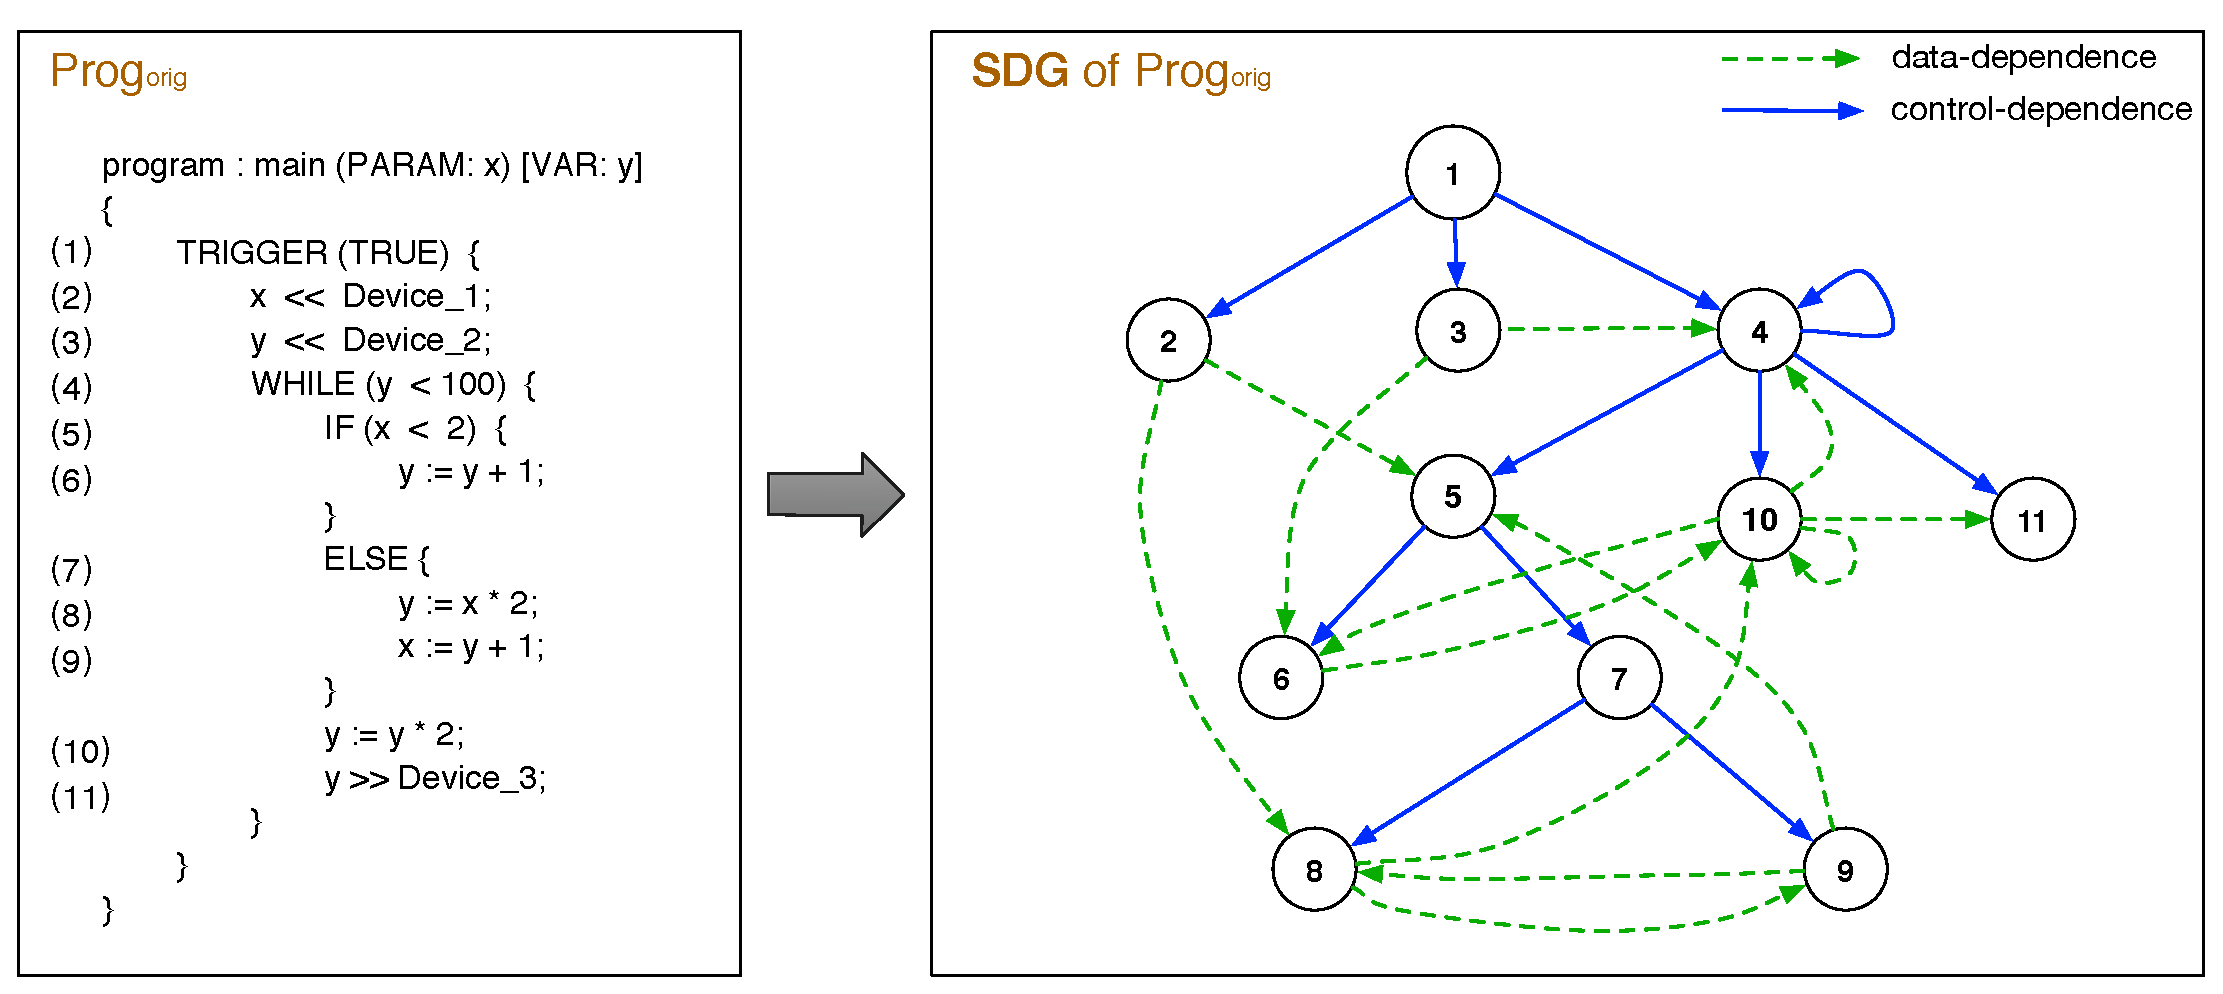
\includegraphics[height=2.1in, width=3.5in]{fig_SDG_exapmle}
    \caption{A example of a simple SDG of $Prog_{orig}$}\label{fig_SDG_exapmle}
\end{figure}


\subsection{Decomposition with Resource Constraints}
This part is to decompose the \emph{Original Model} into \emph{Decomposition Model} with resource constraints. $DD_{pre}$, the \emph{pre} data-dependency for each statement, can be obtained from corresponding $DD_{post}$. The definition is as follows:
\begin{displaymath}
    DD_{pre}(j) \ = \ \{ i \ | \ j \in DD_{post}(i), \ \forall i, j \in N \}
\end{displaymath}
where $j$ is a statement that data-depended on the statement in $DD_{pre}(j)$.
% For example, $DD_{pre}(j) = \{2, 7\}$ means that the statement $j$ are data-depended on statement $2$ and $7$.


The $Algorithm $ \ref{alg:SDGtoDecomposition} presents the principal procedures of the decomposition algorithm.
It includes two \textbf{inputs}:
\begin{enumerate}
  \item SDG: \ The system dependence graph of \emph{Original Model} and every node in the tree is a statement with \emph{REF(node)}, \emph{DEF(node)} and \emph{INFL(node)}.
  \item resConst: \ A mapping of resource constraints to $CU$.
\end{enumerate}
The \textbf{output} in this algorithm is \emph{decompModel}, which is a $Decomposition \ Model$ with all statements labeled by specified $CU$.

The core of this \textbf{Algorithm \ref{alg:SDGtoDecomposition}} comprises three steps:
\begin{enumerate}
\item Firstly, if one statement is associated with one resource, we label the statement with $CU$ corresponding constraints of this resource.
\item Secondly, for every statement $n$ labeled with \emph{CU}, we will label the same $CU$ for every statement in $DD_{pre}(n)$ that has not been labeled, which can ensure the influence on the decomposition for every resource as fair as possible.
\item After the two steps above, there are still some statements have not been labeled, then we label them with the $CU$ in their forward control-dependence statement. It indicates that if there are statements $n$ and $m$ in \emph{INFL(n)} , then the $m$ will be labeled with $CU$ in $n$.
\end{enumerate}


\begin{algorithm}[!htb]
\SetKwInOut{Input}{input}
\SetKwInOut{Output}{output}
\SetKwProg{Fn}{function}{}{}
\SetKwFunction{expandLabels}{expandLabels}
%\DontPrintSemicolon
% \tiny\tiny\scriptsize\footnotesize\small\normalsize\large\Large\LARGE\huge\Huge\footnotesize\small\normalsize\large\Large\LARGE\huge\Huge
% \liuhao
\small
\label{alg:SDGtoDecomposition}
    \caption{Decompose model with the Resource Constraints.}
    \KwIn{ (1) The \textbf{SDG} of system;\\  \ \ \ \ \ \ \ \ \ \ (2) The \emph{Resource Constraint}, \textbf{resConst};}
    \BlankLine
    \KwOut{(1) The $decompModel$ that all statements are labeled with specified $CU$;}
    \BlankLine
    \BlankLine

    $Set\langle Resource \rangle$ R = \{res $|$ res $\in$ resMap.keySet() \}\;
    \For{all $n$ $\in$ $N$}
    {
       $decompModel$.set(n, $\varnothing$)\;
       \For{ all $res$ $\in$ R}
       {
            \If{$res$ $\in$ \emph{REF(n)} $||$ $res$ $\in$ \emph{DEF(n)}}
            {
                $decompModel$.set(n, resmap.get(res))\;
            }
       }
    }

    \For {all $n$ $\in$ $N$}
    {
        $expandLabels$(n, $DD_{pre}(n)$)\;
    }

    \For {all $n$ $\in$ $N$}
    {
        $expandLabels$(n, \emph{INFL(n)})\;
    }

    \Fn{\expandLabels{Int current, $Set\langle Int \rangle$ $Dep$}}
    {
        \For{all $m$ $\in$ $Dep$}
        {
            \If{$decompModel$.get(m) = $\varnothing$}
            {
                $decompModel$.set(m, resmap.get(m))\;
            }
        }
    }
\end{algorithm}

%$decompModel(i, cu)$ where $i$is denotes a statement, and $cu$ is a \emph{CU label}.
% decompModel(i, cu)例子
% i : 1, 2, 3, 4
% cu: A, B, A, C

%% 算法复杂度介绍
% 在算


In this algorithm \ref{alg:SDGtoDecomposition}, the algorithm can be summarized that requires $\mathcal{O}(|N||R|+2|N||Dep|)$ time, and $\mathcal{O}(|N|+|R|+|DD_{pre}|+|INFL|)$ space.


